\documentclass{beamer}

\usepackage[T1]{fontenc} 
\usepackage[latin1]{inputenc}
%% \usepackage[frenchb]{babel}

\usetheme{Warsaw}

% Supprimer les icones de navigation (pour les transparents)
\setbeamertemplate{navigation symbols}{}

\title[Presentation BioSilico Base]{Presentation BioSilico Base}
\author{Gabriel Chandesris}
%% \institute{ --- }
\institute{ 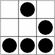
\includegraphics[height=0.5cm]{../img/logo_glider.png} }
%% \logo{ 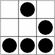
\includegraphics[height=2.5cm]{../img/logo_glider.png} }
\date{\today } %% \date{\today}

\begin{document}

\begin{frame}
	\titlepage
\end{frame}

\begin{frame}
	\frametitle{Table Of Content}
	\small \tableofcontents[hideallsubsections]
\end{frame} 

\def\titleSectionCurriculumPart{Curriculum Part}
\section{\titleSectionCurriculumPart }
\begin{frame}
	\frametitle{\titleSectionCurriculumPart }
	\tableofcontents[sections=1,currentsection,subsectionstyle=show/shaded/hide]
\end{frame} 

\def\titleSubSectionCurriculumPartOne{Starting points}
\subsection{ \titleSubSectionCurriculumPartOne }
\begin{frame}
	\frametitle{ \titleSubSectionCurriculumPartOne }
	\begin{columns}[T]
	\begin{column}[T]{6.0cm}
		\begin{block}{What I Wanted to do}
			\begin{itemize}
				\item Major interest for Computers and related Tools ; 
				\item Interest for Science and Biology ; 
				\item Experimentations in both domains ; 
				\item[] 
				\item Curiosity ! (and some ideas)
			\end{itemize}
		\end{block}
	\end{column}
	\begin{column}[T]{5.0cm}
		\begin{block}{Diplomas (``French Intitul{\'e}s'') }
			\begin{itemize}
				\item \textbf{2000} Baccalaur{\'e}at Scientifique Sp{\'e}cialit{\'e} Sciences de la Vie et de la Terre ; 
				\item \textbf{2003} BTS Biochimiste ; ~\\
				Training: ``\emph{Diagnostic de l'h{\'e}mochromatose g{\'e}n{\'e}tique par biologie mol{\'e}culaire -- Validation d'une technique automatis{\'e}e}''
				%% \item ... \emph{the following in next slides !}
			\end{itemize}
		\end{block}
	\end{column}
	\end{columns}
\end{frame} 

\def\titleSubSectionCurriculumPartTwo{Continuation (working and studying on same time)}
\subsection{ \titleSubSectionCurriculumPartTwo }
\begin{frame}
	\frametitle{ \titleSubSectionCurriculumPartTwo }
	\begin{itemize}
		\item Working as Lab Technicien / Engineer (medical analysis) ; 
		\item Night class in \emph{Conservatoire National des Arts et M{\'e}tiers} ; 
		\item Certification (2005) then Licence (2007) in BioInformatics 
		(training at Sanofi R\&D SCDM : a data integration module)
		\item[]  
		\item \textbf{2009} Master of BioInformatics at Evry (near Genopole)
		\begin{itemize}
			\item Train on Year 1 : IBISC CNRS Lab at Evry ("Industrialisation d'un logiciel pour la pr{\'e}diction de structures secondaires d'ARN non codants")
			\item Train on Year 2 : Dassault Syst{\`e}mes ("F{\'e}d{\'e}ration de bases de donn{\'e}es en sciences de la vie -- Conception et mise en place d'un prototype dans ENOVIA V6")
		\end{itemize}
	\end{itemize}
\end{frame}

\end{document}
